\section{Anomaly Detection Methods}

As part of the data reduction procedure, a moving average was applied to data in both the time domain and the frequency domain. A moving average essentially applies a low-pass filter to the data. 

For the time domain, this was mainly applied in order to ensure more accurate reconstructions when using techniques such as K-mean Clustering Reconstruction (see \S~\ref{subsec:kmeans}) and LSTM Recurrent Neural Networks (see \S~\ref{subsec:LSTM}).

For the frequency domain, the moving average was applied to the frequency domain, after the Fourier transform has already been applied to the unaltered time series data. This ensures that all of the higher frequencies were not lost.

The method of taking a moving average is implemented using the convolution of the data with a kernel, $k$. If a moving average with width $w$ is required, the kernel is defined as 

\begin{equation}
    k = \big[ \big
    \label{eq:conv_kernel}
\end{equation}


\begin{figure}[t]
    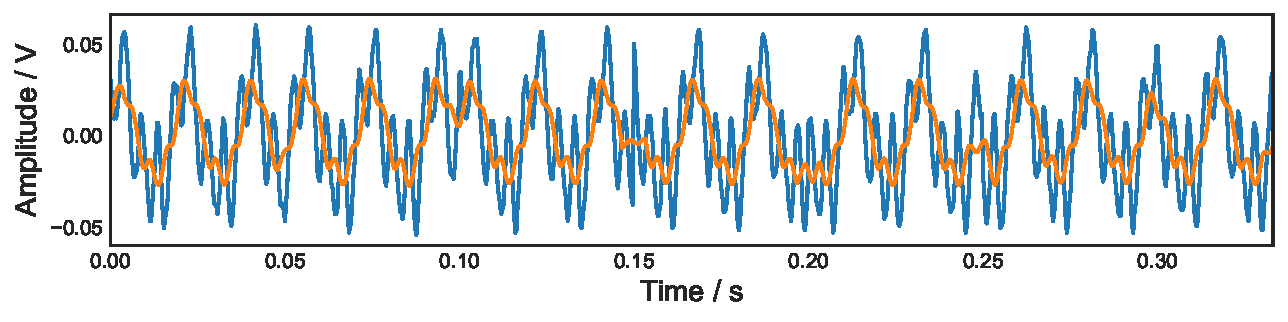
\includegraphics[width=1.0\textwidth]{fig/moving_average.pdf}
    \caption[Time Domain]{Moving average applied to data in the time domain. The original data (shown in blue) represents the amplitude of the signal as a function of time. The orange curve shows the moving average of this data.}
    \label{fig:moving_av}
\end{figure}

\begin{figure}[t]
    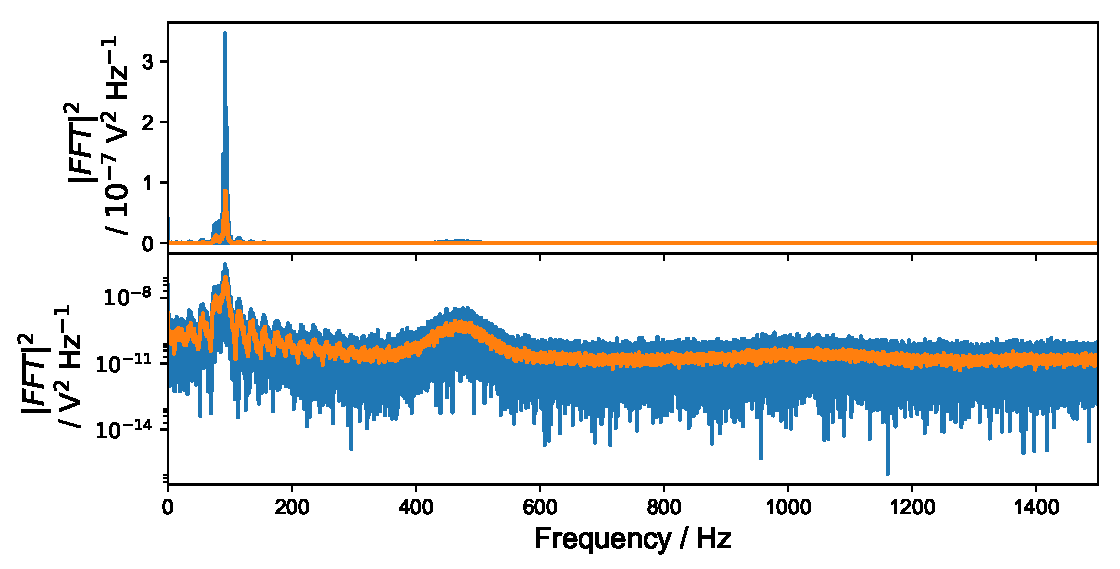
\includegraphics[width=1.0\textwidth]{fig/freq_moving_average.pdf}
    \caption[Fourier Domain]{Moving average applied to data in the Fourier domain, shown in both linear and logarithmic axes. The blue lines show the original amplitudes as a function of frequency. The orange lines show the moving averages.}
    \label{fig:freq_moving_av}
\end{figure}


\subsection{Statistical Approach}

The most simple methods for detecting changes from `normal' motor behaviour can either use simple value thresholds, or static mean and standard deviation calculates to determine when data experiences a significant deviation from usual patterns. 

Such basic approaches are not easily adapted for use in time series data. This is because:

\begin{enumerate}
    \item These methods are not easily applied to changing data values.
    \item They cannot scale easily to large time series.
    \item An unacceptable quantity of false anomalies can be detected.
\end{enumerate}

As such, our most rudimentary anomaly detection methods take a more statistical approach...

Assume behaviour is normally distributed so that the probability $p$ of a value $x$ is,

\begin{equation}
    p(x) = \dfrac{1}{\sigma \sqrt{2\pi}}\exp(\dfrac{-{(x-\mu)}^2}{2\sigma^2})~,
\end{equation}

where $\mu$ and $\sigma$ are the mean and standard deviation of the sample respectively.

\subsubsection{Histogram Test}

One example would be Histogram Based Outlier Score (HBOS)

\begin{figure}[t]
    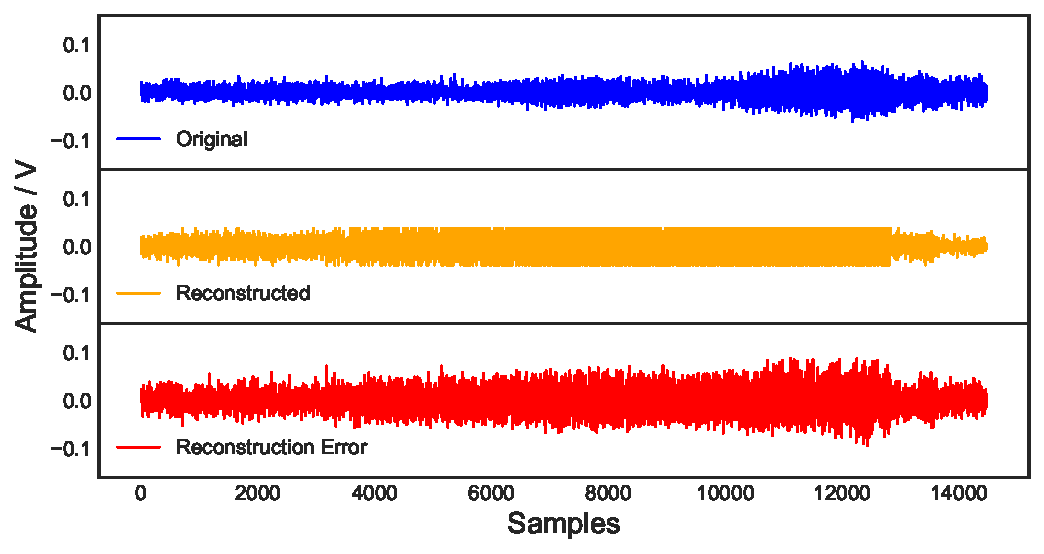
\includegraphics[width=1.0\textwidth]{fig/histogram.pdf}
    \caption[Histogram]{Histogram method}
    \label{fig:histogram}
\end{figure}

\subsubsection{Grubbs' Test}

\subsubsection{Deviation from median}

\subsubsection{Deviation from moving average}

\subsection{Fourier Analysis}
\subsubsection{Lorentzian fitting in frequency space}

 \cite{IJIRD44249}

\subsection{Machine Learning}
    \subsubsection{ARIMA}

\subsubsection{K-Means Clustering}
\label{subsec:kmeans}

K-means clustering is one of the most highly used cluster analysis methods, due to it being much less computationally expensive in comparison to other approaches \cite{Kanungo:2002:EKC:628329.628801}

The process involves partitioning a set of n-dimensional data points, $\{\underline{x}\}$ into a group of $k$ clusters, where $k$ has to be specified by the user. K-means aims to find the centroids $\underline{\mu}_i$, ($i=1...k$), of the clusters that minimise the Euclidean distance from all data points to their respective clusters, $d(\underline{x}, \underline{\mu}_i) = ||\underline{x}-\underline{\mu}_i||^2$. More formally, K-means clustering finds the centroids of $k$ clusters in order to minimise the expression \cite{596afe3f2b5a4ff3b8f4f9793ad2f4ee},

\begin{equation}
    arg\,min_k \sum_{i=1}^{k} \sum_{\underline{x} \epsilon c_i} ||\underline{x}-\underline{\mu}_i||^2 ~,
    \label{eq:K-means}
\end{equation}

where $c_i$ are the points closest to the cluster $i$.

The general process is described as follows:
\begin{enumerate}
    \item Initialise the centre of the $k$ clusters randomly in Euclidean n-space.
    \item Attribute each data point to the closest cluster centre for that data point. 
    \item Assign a new position for the cluster centre, now given by the barycentre of the data points belonging to the cluster.
    \item Repeat steps 2 and 3 until convergence to a solution is achieved.
\end{enumerate}

An example to illustrate clusters 2 dimensions is shown in figure(MAKE FIGURE!). 

-------How K-means was used for our data


Talk about semi-supervised K-means and why this method is semi-supervised rather than unsupervised \cite{596afe3f2b5a4ff3b8f4f9793ad2f4ee}.

\begin{figure}[t]
    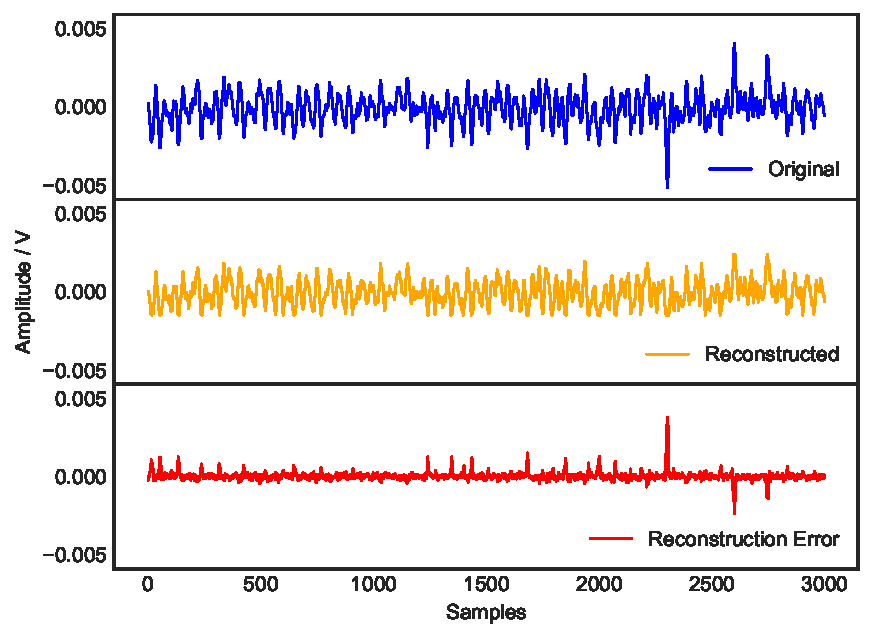
\includegraphics[width=1.0\textwidth]{fig/kmeans.pdf}
    \caption[K mean clustering plot]{Fancy figure goes here.}
    \label{fig:kmeanerror}
\end{figure}

\subsubsection{LSTM Recurrent Neural Networks}
\label{subsec:LSTM}

Machine learning is the science of programming computers in a manner that means they carry out tasks while not being explicitly programmed. In the past decade, machine learning has given us self-driving cars, practical speech recognition, effective web search, and a vastly improved understanding of the human genome.

First proposed by \cite{Hochreiter:1997:LSM:1246443.1246450}. Overcome the `vanishing gradient' problem. 
\begin{figure}[t]
    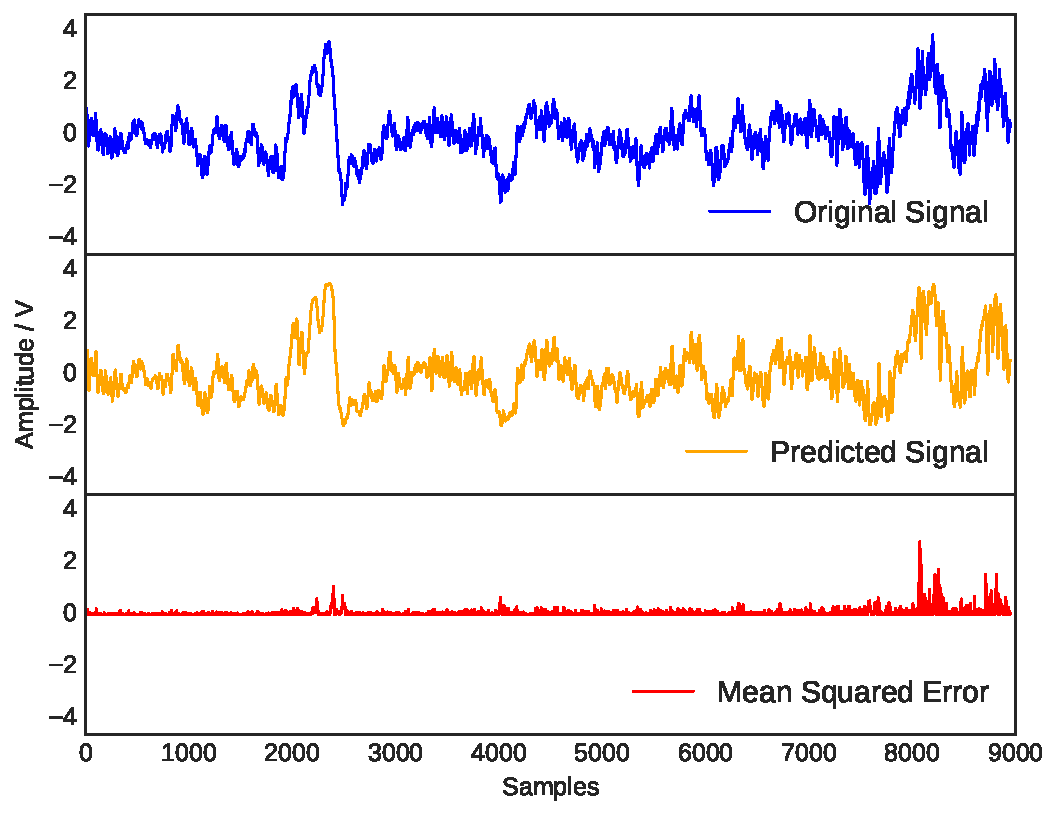
\includegraphics[width=1.0\textwidth]{fig/neuralnetwork.pdf}
    \caption[Neural Network]{Using the LSTM funtionality provided by \texttt{Keras}.}
    \label{fig:kmeanerror}
\end{figure}
